\documentclass[11pt]{article}
\usepackage[utf8]{inputenc}
\usepackage{amsmath}
\usepackage{amsfonts}
\usepackage{amssymb}
\usepackage{graphicx}
\usepackage[super]{nth}
\usepackage{amsthm}
\newtheorem{theorem}{Theorem}
\newtheorem{objective}{Objective}
\newtheorem{model}{Model}


\makeatletter
\renewcommand{\maketitle}{
\begin{center}

\pagestyle{empty}
\phantom{.}  %necessary to add space on top before the title
\vspace{3cm}

{\Huge \bf \@title\par}
\vspace{2.5cm}

{\LARGE Marcel Gietzmann-Sanders}\\[1cm]

{\Large\@date}

\vspace{2.5cm}
{\Large Dr. Andrew Seitz}\hspace{2cm}{\Large Dr. Curry Cunningham}\\[2cm]{\Large Michael Courtney, M.S.}\\[2cm]
College of Fisheries and Ocean Sciences\\
University of Alaska Fairbanks


\end{center}
}\makeatother


\title{Master's Research Proposal (DRAFT)}

\date{2024}
\setcounter{tocdepth}{2}
\begin{document}
\maketitle
\newpage

\section{Navigating This Document}

This document is organized in order to allow you, the reader, to read as little or as much as you need/want. \newline

It begins with the \textbf{objectives} so that you immediately know exactly what this proposal is hoping to achieve and whether this is of interest to you.  \newline

Then it dives into how we will go about demonstrating success in those objectives. This will inform you on the specific \textbf{outcomes} to be expected. \newline

Finally there is a \textbf{timeline} provided to give a sense of when these outcomes can be expected. \newline

If these sections are compelling enough there is no need to read any further. \newline

However if you are interested in the rationales behind these objectives or diving into the related context, the \textbf{Rationale} and \textbf{Related Context} sections are for you. 

\newpage


\tableofcontents
\newpage

\section{Objectives}

The ultimate goal of this research is to provide a new pathway by which collections of high resolution spatio-temporal movement data that are representative of a species can be used to make a direct impact on fisheries management. It is hoped that this will provide an incentive for creating/enlarging such datasets. 

\begin{objective}
To provide tooling that allows for using machine learning methods to fit models of the form

$$\psi_k = G(\eta_k)$$

that maximize the following objective:


$$\mathcal{L}=\prod_i P'(v_i | \eta_i)$$

where:

$$P'(v_i|\eta_i) = \frac{\psi_i}{\sum_k \psi_k}$$

These models will be known as odds models as they predict the "odds for" each outcome $v_k$ given the information contained in $\eta_k$. 

\end{objective}

\begin{objective}
To provide tooling that allows for running spatio-temporal simulations of management strategies using movement models as defined above. Such simulations should allow for:

\begin{enumerate}
\item Flexible initial assumptions that capture heterogeneity in the stock.
\item The ability to impose spatio-temporal mortality (both fishing and natural).
\item The ability to capture heterogeneity in fishing vulnerability.
\end{enumerate}

Likewise these simulations need to be quick enough to allow for capturing uncertainty in initial conditions through bootstrapping.\newline

These simulations will be known as diffusion models as they model the probabilistic behavior of cohorts as opposed to individual fish or schools. 
\end{objective}



\newpage


















\section{Demonstrations}

Our demonstrations of the above objectives will be split into two chapters. 

\subsection{Chapter 1}

Chapter 1 will be concerned with demonstrating the tooling for creating odds models for spatio-temporal movement behavior. It will pursue two specific modeling examples:

\begin{model}
A depth occupancy model for Chinook salmon in the Gulf of Alaska (GOA). \newline

\textbf{Target:} Depth range. \newline

\textbf{Features:} Environmental data derived either from environmental simulations or from remote sensing such as Google Earth, cohort data about the fish themselves, and temporal features such as month, season, or time of day. \newline

\textbf{Data:} PSAT tagging data from the GOA. \newline 

\textbf{Purpose:} To study the heterogeneity in depth occupancy as a function of cohort, environment, and time.  
\end{model}

\begin{model}
A movement model for Chinook salmon in the Gulf of Alaska (GOA). \newline

\textbf{Target:} Spatial grid cell selection as movement. Any state feature updates needed to capture internal states of a cohort. \newline

\textbf{Features:} Environmental data derived either from environmental simulations or from remote sensing such as Google Earth, cohort data about the fish themselves, temporal features such as month, season, or time of day, and internal state information about the cohort. \newline

\textbf{Data:} PSAT tagging data from the GOA. \newline

\textbf{Purpose:} To study the heterogeneity in spatial movement/preference as a function of cohort, environment, and time.\newline

\end{model}

In building these models our primary purpose is to demonstrate the tooling exists to prudently build odds models. We can frame this goal in terms of a "standard" machine learning pipeline and work-flow. 

\begin{enumerate}
\item Formatting Data for Odds Modeling 
\item Class Balancing
\item Splitting Data into Train, Validation, Test
\item Training and Hyperparameter Tuning Using Standard Model Types
\item Diagnoses of Fit and Comparison of Different Model Types
\item Identifying Sample Groups that are More or Less Fit
\end{enumerate}

We will want to explicitly demonstrate each of these processes, provide guidance on using the tools for them, and use them to build the models listed above. \newline

The outcome will be a package in Python for building, diagnosing, and running odds models.

\subsection{Chapter 2}

Chapter 2 will be concerned with taking these models for Chinook salmon in the Gulf of Alaska and building a spatio-temporal movement simulation that can be used to investigate a series of management questions. It is worth noting that we will use the simulation to ask questions that may come up in general management settings even if they may not be directly applicable to the issues currently faced by Chinook salmon management in the GOA. This is just to demonstrate general applicability. \newline

The overview of the components of this simulation are outlined in Fig. \ref{fig:simulation}. 

\begin{figure}[h!] 
  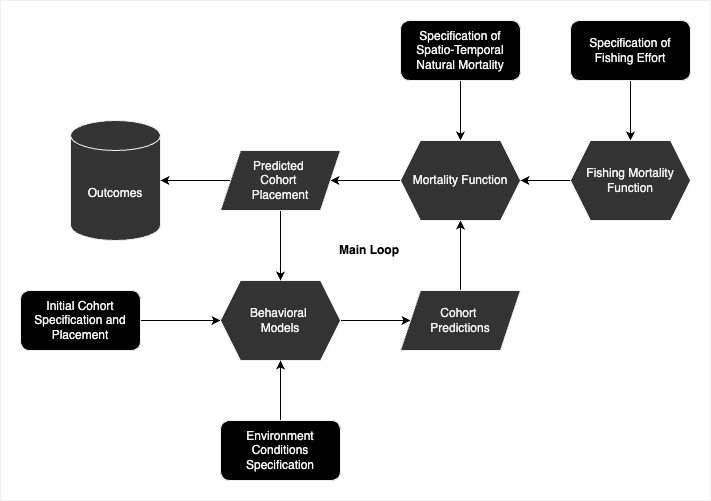
\includegraphics[width=\linewidth]{simulation.png}
  \caption{Simulation Outline}
  \medskip
	\small
	Boxes with rounded edges would be inputs specified by the user. The hexagons are functions 		provided by the simulation and the trapezoids are data generated during the main loop. 
  \label{fig:simulation}
\end{figure}


Some specific use cases we want to demonstrate with this simulation are:

\begin{enumerate}
\item \textbf{Understanding Connectivity:} by looking at the vector flows of fish throughout the space we will be able to identify which areas are highly connected and which are more or less separated by environment, cohort, or other factors of fish behavior.
\item \textbf{Understanding Vulnerability:} by especially looking at changes in depth occupancy and preference for habitat we will attempt to quantify the degree of vulnerability to different kinds of fishing gear as a function of space and time. 
\item \textbf{Cumulative Mortality:} by being able to follow cohorts through space and time we should be able to show how different fishing pressure scenarios affect the cumulative fishing mortality.
\item \textbf{Protected Areas/Times:} Of those fishing pressure scenarios, one of especial interest is modeling Marine Protected Areas (MPAs) or other kinds of closures in space and time.
\item \textbf{Uncertainty:} we will show that such a simulation can be run at scale, bootstrapping can be applied, and therefore uncertainty in simulation outcomes quantified. 
\end{enumerate}

To give a specific example of what this might look like in practice, if we were interested in understanding how to protect one specific genetic cohort by creating fishing closures we would:

\begin{enumerate}
\item Input a distribution of the cohort at some initial time point as relative abundance per spatial grid cell.
\item Input a time period over which to run the simulation (perhaps the fishing season in the area under study).
\item Collect and input any environmental data needed for the movement model indexed by space and time.
\item Then we might run the simulation without any fishing pressure to understand how the cohort naturally distributes itself and generate hypotheses for closures from this.
\item We could then input fishing pressure (as a mortality function) by space and time for a few different scenarios where some would include our closures.
\item Run the simulation for each of these scenarios and compare resulting abundance trends. 
\end{enumerate}

The outcome will be a package in Python for deploying, running, and analyzing diffusion models. 





\newpage



\section{Timeline}

\subsection{Class Work}

\begin{enumerate}
\item \textbf{Fall 2023:} (University of Florida) FAS 6355c Fisheries Management, FAS 6337c Population Dynamics
\item \textbf{Spring 2024:} FISH F621 Estimation of Fish Abundance, FISH F427 Ichthyology
\item \textbf{Fall 2024:} STAT F641 Bayesian Statistics, FISH F692 Seminar
\item \textbf{Spring 2025:} FISH F631 Data Analysis in Community Ecology, FISH 699 Thesis 
\item \textbf{Fall 2025:} STAT F651 Statistical Theory I, FISH 699 Thesis
\item \textbf{Spring 2026:} FISH F626  Behavioral Ecology of Fishes, STAT F605 Spatial Statistics 
\end{enumerate}

\subsection{Thesis}

\begin{enumerate}
\item \textbf{Spring 2024:} Depth and Movement Models v0, Thesis Exploration
\item \textbf{Fall 2024:} Graduate Study Plan, Self Evaluation, Thesis Proposal, Depth and Movement Models v1
\item \textbf{Spring 2025:} Thesis Proposal Defense, Simulation v1
\item \textbf{Fall 2025:} Self Evaluation, Write Chapters, Publish Package(s)
\item \textbf{Spring 2026:} Thesis Defense
\end{enumerate}

\newpage


















\section{Rationale}

\subsection{Objective 1} \label{objective1}

\subsubsection{Value of Machine Learning in Model Building}

One of the functions of science is to build models of the world around us, specifically to look for functions of the form:

$$v=F(\theta)$$

where $\theta$ is some vector of information, $v$ is a particular outcome given that information, and $F$ is the model in question. This we might term a \textit{deterministic model} because for any specific $\theta$ there is one single outcome $v$. 

However, life is rarely so kind to us. From quantum physics to fisheries science, the world is replete with examples where the same information does not always lead to the same conclusion. Sometimes that is because we do not possess all of the relevant information but sometimes things are just truly random. As such, the model above will in some sense be lying to us in its deterministic certainty - while we will always predict $v$, $v$ is not always what we will receive. 

Instead suppose that for a specific $\theta$ there exist a set of possible outcomes $V(\theta)=\lbrace v \rbrace$. We can define a \textit{stochastic model} as:

$$P(v|\theta)=F(v, \theta)$$ 

where now the model is predicting the probability of $v$ given $\theta$ instead of just predicting $v$ itself.

Now what is especially interesting about models of this form is the fact that in some sense for any combination of $V$ and $\theta$ they always exist. Whereas to get a deterministic model we need to know precisely what kind of information ($\theta$) we need to make a deterministic prediction, we can always make a stochastic one, even in the presence of no information. The model can always give us a correct answer, it's just a question of how useful that answer is. If you base it off of better data it will become more useful.

Unfortunately, unless we ourselves have built the part of the world we're studying, $F$ is not known to us. Instead our models are really just proposals $\hat{F}$ on what $F$ could be. This presents us with an immediate problem, how do we evaluate any specific $\hat{F}$ if we don't know $F$ itself? Well suppose we've captured a whole series of pairs of $\theta_i$ and $v_i$ where $i$ allows us to index the pair in question. Given we know $\hat{F}$ we can directly ask what the likelihood of the data we have collected is, given $\hat{F}$:

$$\mathcal{L}=\prod_i \hat{F}(v_i, \theta_i)$$

or equivalently (and more easily computed)

$$\ln \mathcal{L} = \sum_i \ln \hat{F}(v_i, \theta_i)$$

$\hat{F}$'s with higher $\ln \mathcal{L}$ (log likelihood) are better fits to the given data and as we have more and more comprehensive data those data better and better represent $F$ (see Appendix 1).

Therefore finding the "true" $F$ can be summarized with two steps:

\begin{enumerate}
\item Collect large amounts of comprehensive data.
\item Find the $\hat{F}$ that maximizes the likelihood of that data.
\end{enumerate}

All of this, however, has been conditional on the form of $\theta$ having been chosen. Obviously, the information we choose to collect and build our model with has an impact on how good the model is from a purely predictive perspective. So how can we compare the predictive power of different $\theta$? Well as we find $\theta$ that are more predictive the corresponding $F$s will have greater and greater likelihoods $\mathcal{L}$, given the data. But this presents us with a chicken and the egg style problem - to know the value of $\theta$ we must know $F$, but to know $F$ we must have fit $\hat{F}$ which requires a reasonable amount of data to have been collected. I.e., we cannot know in advance if the data we are collecting is going to be useful or not. Instead anyone doing modeling finds themselves in the cycle (Fig. \ref{fig:model_cycle}).

\begin{figure}[h!] 
  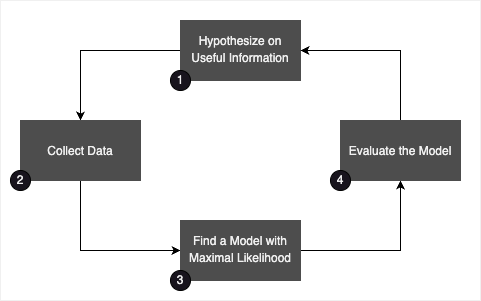
\includegraphics[width=\linewidth]{model_cycle.png}
  \caption{Modeling Cycle}
  \medskip
	\small
	The four major steps in building good models. Note that while one must always start at (1) this process is indeed a cycle.
  \label{fig:model_cycle}
\end{figure}

Each step in this cycle is highly non-trivial. However special interest should be paid to step 3 (finding an $\hat{F}$ that best approximates $F$). 

The standard method here has been to propose a family of possible $F$ which are defined by a set of parameters $\mu$. Then using some choice of likelihood maximization method the set of $\mu$ are searched for that maximize the likelihood of the data $\mathcal{L}$. While this method has borne considerable fruit it still requires a great deal of effort on the side of the scientist to envision various hypotheses on what families of functions would make sense, coding those up, fitting them, and then evaluating them post-fit. Furthermore if the true form of $F$ is not contained in those set of hypotheses tested then $F$ is never found. Lots of effort without any kind of guarantee that $F$ will be discovered.  

The field of Machine Learning (ML) (specifically probabilistic machine learning) on the other hand has been specifically occupied with finding ways to maximize objectives without having to assume much, if anything, about the functional form of the prediction function. Therefore it provides an opportunity to lessen the toil and uncertainty in step 3 and allow scientists to focus more of the efforts on the other steps (and thereby accelerate the whole cycle).

\subsubsection{Issues with Probabilistic Machine Learning when Applied to Behavior}

Probabilistic machine classification \cite{durr} of the kind we were pointing to in the last section has two pitfalls when it comes to modeling behavior. 

The first comes from the fact that such models predict on the same set of outcomes each time, regardless of $\theta$. For example, if we were trying to predict which drink a person will buy at their local cafe we would not only have to include everything currently on the menu but also everything that could be on the menu across all time points we are interested in predicting. If suddenly a new menu item appears that we have not trained on, our probabilistic classifier will be at a loss. 

The second issue comes from the "curse of dimensionality." Basically this is an issue where as the dimensionality of $\theta$ increases, the amount of data required to find real relationships in that data increases exponentially. This is a particular problem for behavioral modeling because we in all likelihood need to include data on each of the possible decisions before us. So if I can choose between five different drinks I need to provide features on each of those five drinks. This leads to very high dimensional spaces very quickly. \newline


We can get around both of these problems by introducing what we will term an "odds model." Specifically if we imagine $\theta$ now as a variable length vector composed of vectors $\eta_k$ for each of our possible outcomes $v_k$ then the odds model is given by the function:

$$\psi_k=G(\eta_k)$$

where we now say that:

$$P'(v_k|\theta) = \frac{\psi_k}{\sum_j \psi_j}$$

We can see why we chose the name "odds model" as the $\psi_k$ are simply the "odds for" outcome $v_k$. \newline

Now note it is not necessarily true that:

$$P'(v_k|\eta_k) = P(v_k|\theta)$$

because it is possible that information in the other $\eta_j$ informs the probability of $v_k$. However it should be possible to include such information in the $\eta_k$ if necessary. 

By making this sacrifice, however, we have achieved two things:

\begin{enumerate}
\item So long as we can provide a $\eta_k$ for a newly seen outcome we can predict on it. Therefore we need not have a fixed set of possible outcomes (or a fixed number of such outcomes per $\theta$).
\item Compared to the corresponding probabilistic machine learning classifier, if our total number of outcomes were $|V|$ we've now reduced the dimensionality of our feature space by $|V|$. 
\end{enumerate}

And this means that unless we have to pass large amounts of information between the $\eta_k$ the amount of data we need to collect to fit our model has decreased tremendously. And in cases where data is hard to come by (like animal behavior), any reduction in data requirements is of the utmost importance. 

So finally, to model behavior we'd like to fit an odds model of the form:

$$\psi_k = G(\eta_k)$$

that maximizes:

$$\mathcal{L}=\prod_i P'(v_i | \eta_i)$$

where 

$$P'(v_i|\eta_i) = \frac{\psi_i}{\sum_k \psi_k}$$\newline









\subsection{Objective 2}

From studies that started with Beverton and Holt's work on recruitment in fisheries, we know, with a reasonable degree of certainty, that as a general rule fish stocks operate according to an asymptotic relationship between spawning biomass and recruits \cite{waltersmartell} (Fig. \ref{fig:recruitment}). What we see is a clear pattern in recruitment verses spawners for low spawners and then eventually we reach a point where this curve asymptotes and large changes to the number of spawners creates little to no change (especially when considering the actual variability in this data) in the number of recruits. Obviously, given the real variability in nature, this pattern looks more like a scatter shot of points but plenty of studies over several species have shown this overall pattern in the mean borne out \cite{waltersmartell}. \newline

\begin{figure}[h!] 
  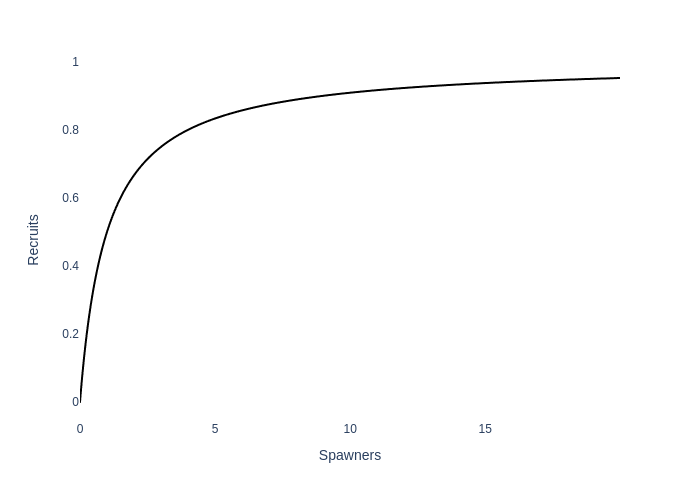
\includegraphics[width=\linewidth]{recruitment.png}
  \caption{Recruitment}
  \label{fig:recruitment}
\end{figure}



The implication for fisheries management is pretty clear - sustainable fishing is in large part driven by just maintaining the spawning stock biomass (SSB) above that knee in the curve \cite{waltersmartell} \cite{king}. Indeed this is well noted as the basis of why fisheries \textit{can} exist in the first place. If taking spawners always led to decreases in recruits, we'd quickly fish a stock out of existence. It is only through the compensation we get on the asymptote that sustainable fisheries are possible. \newline

However, two very simple observations of fish biology will show how actually managing SSB can be made difficult.

The first, and simplest, is age structure. Obviously we're talking here about maintaining a specific level of spawning stock biomass. But today's juveniles are tomorrow's SSB and as fish grow they typically become more fecund. This means that in order to maintain our SSB over time we have to be careful about how we target each age group. This gets even more complicated for fish like Pacific salmon (\textit{Oncorhynchus}) or many species of groupers (\textit{Epinephelinae}) where life history is intimately entwined with spawning. The salmon obviously only breed once \cite{NOAA24} and some species of groupers are protogynous hermaphrodites \cite{RedGrouper} meaning that if you target a specific age group you are effectively targeting a specific sex. Clearly understanding and managing our age class selectivity matters when it comes to maintaining a healthy SSB for years to come. \newline

The other observation is that many species of fishes actually form multiple sub stocks within what we may consider a single fishery (or sometimes many fisheries distributed across different countries) \cite{lorenzen2010} \cite{salmonplan} \cite{prince2010}. Pacific salmon are once again a good example in that they home to specific streams and only breed with other salmon in those streams and many other species of fish form fish spawning aggregations as well \cite{erisman2017}. Research also indicates that even fish like Atlantic herring likely form distinct genetic groups due to differences in homing during breeding and school behavior \cite{armstrong2001}. 

What does this mean? It means that if we trust our Beverton-Holt style model, instead of having a single SSB to manage we really have several SSBs - one for each sub stock. Obviously, if we set one global piece of management like an Allowable Biological Catch (ABC) that makes sense for a single SSB but then have biased fishing mortality where one sub stock is getting fished out far more than the others we may drop below the SSB for that one stock without actually exceeding our expected ABC for the whole fishery. And this can certainly happen as different sub stocks will often exhibit quite different spatial behaviors in movement \cite{tucker2019} \cite{punt2019} \cite{cadrin2020}. \newline

All of this to say that understanding heterogeneity in vulnerability by things like age class and sub stock is of the utmost importance for managing a fishery and truly ensuring an appropriate amount of SSB remains year over year. It is also worth noting that this knowledge around changes in selectivity in space and time is not only useful for considerations around SSB but also for other management issues such as bycatch avoidance and growth overfishing. 

What kind of tooling do we need in order to address these issues and test out ideas for "selectivity aware" fisheries management? Clearly we need some kind of reliable simulation. \newline

Suppose we built models of spatio-temporal behavior (specifically movement) as expressed in Objective 1. These models we know can be fed information that captures both environmental variables but also factors we'd like to categorize by in order to understand heterogeneity in selectivity. Such variables could include features like the age and genetic cohorts that we just described. Then we could take some baseline assumptions about abundance in space at a given time (say providing recruits at spawning grounds or taking a spatio-temporal assessment as a starting point) and use our behavioral models to simulate time-steps forward. As we do, we could account for natural mortality as well to complete the "environment" portion of our simulation. 

It is important to note that while this may seem like a Lagrangian approach to simulation it actually falls more into the Eulerian camp as, in order to reduce our computational costs, we'd simply have cohorts as a function of space. Remember that our model is only taking the categories that separate one group from the next thereby allowing us to model cohorts instead of single individuals. Furthermore instead of modeling the specific singular behaviors our behavior model as outlined in Objective 1 allows us to understand the "many world" probabilistic outcomes of behavior. We are not following a single fish but instead are watching as that cohort diffuses across its decision space. Therefore we'll term this simulation a diffusion model.

Into our diffusion model we can now incorporate whatever management policy we like as a spatio-temporal specification of fishing mortality - which can now be modulated by our understanding of, say, gear selectivity as a function of space and time. So if we want to implement a marine protected area we can take a baseline fishing pattern and exclude specific areas in space. If we want to see what would happen if we redistribute the fleet we can as well. If we just want to understand the selectivity biases already present we can simulate fleet patterns as they occur today. 

The point is that with such a simulation we are able to test different hypotheses of management on data driven understanding of fish behavior. 


\subsection{PSAT Data}

Pop-up Satellite Archival Tags (PSATs) are a great way of collecting behavior data \cite{PSAT}. They are defined by three key properties:

\begin{enumerate}
\item \textbf{Archival:} Transmitting data is only possible if animals come to the surface. Therefore these tags archive collected data for later transmission. 
\item \textbf{Pop Up:} These tags are programmed to release from a fish at a specific time or under specific conditions to facilitate retrieval. 
\item \textbf{Satellite:} On pop-up the tags then broadcast data (usually summarized) to Argos satellites which is then relayed to a database for retrieval. Such tags usually also broadcast some information that can be used to deduce position as well which allows for direct retrieval and access to the full archived dataset.
\end{enumerate}

The normal lifecycle then is to catch an animal, attach the tag, allow the animal to go about its life all while collecting data, have the tag pop-up, transfer data to satellite or retrieve the tag, and then clean and analyze the data. \newline

For our purposes these tags critically capture:

\begin{enumerate}
\item Temperature
\item Depth
\item Light Levels
\end{enumerate}

The latter two are then used along with tag release location to predict animal movement (latitude and longitude) using a proprietary statistical model \cite{PSAT}. 

We will look at movements on a day by day basis and depths at the transmitted resolution (2-5 minutes). For those tags retrieved, a much higher resolution is available (1-3 seconds) however most data is only guaranteed from transmission and not from retrieval \cite{PSAT}. 
\newline

Clearly then this kind of data suites our modeling and simulation purposes well as we get behavior outcomes directly. 

\subsection{Chinook salmon in the GOA}

At this point in time the main interest here is that Chinook salmon present an interesting model species for testing out the efficacy of these models and simulations. Chinook salmon are highly motile and undergo clear migration behaviors \cite{tucker2019} \cite{langan2024}. Therefore they should provide a good challenge to attempts at behavioral modeling and simulation. It is the author's hope that patterns useful to Chinook salmon management issues may arise from this research but it is not a necessity as the intention here is to develop tools that justify additional data collection for species for which spatial management is of interest. 





























\newpage















\section{Related Context}

\subsection{Summary}

The sum outcome of the work proposed is the creation of a simulation that can be used to explore, propose, and (in simulation) test management options. The advantages of having such a simulation are many (as is described in the following situations) and therefore it comes as no surprise that the notion of using a simulation to drive understanding of management options is in no way novel. Indeed as is demonstrated in the following sections many different kinds of simulation (or analogs) already exist. Assessment paradigms are a form of simulation, movement models based on more traditional tagging methods can be used in simulation, and individual based models of several sorts have lent themselves to simulations used to assess changes to environment or management as well. Therefore the question is - what advantages come from the proposed direction? 

\begin{enumerate}
\item \textbf{Isolating the Study of Movement (\S \ref{spatial_assessments}).} In machine learning there is a well known phenomenon where features that are even mildly correlated with one another can compensate for one another in model fitting. A simple example would be something like height representing the "feature impact" of sex in a model of human health. Therefore it is always dubious to treat the relationship between a feature and a target as an actual indication of the true relationship. Within the spatial assessment paradigms in use today many different parameters of life history are fit together - movement, spatial heterogeneity in recruitment or mortality, fishing pressure, and so on. Because these are all fit as one model it is possible if not likely that features are "compensating" for one another and obscuring the actual relationships between the underlying processes and the outcomes. The simulation proposed herein fits movement on its own which should lead to a greater confidence in its representation of actual fish movement patterns. It also makes the debugging and improvement of those models much more clear and straightforward. 
\item \textbf{Generalized Strategy (\S \ref{modeling_movement}).} Individual based models (IBMs) also solve the problem mentioned above as they directly model movement as well. However IBMs are notoriously specific to the problem at hand. Furthermore most IBMs represent a specific hypothesis of behavior that has been coded up and as was mentioned in Section \ref{objective1} building models this way takes an enormous amount of time. The strategy proposed herein provides a generalized tool set for going from data, to a model, and then from there to a spatial simulation. And this means that researchers can contribute to building up a common tool set instead of having to start from ground zero each round.
\item \textbf{Repeated Usefulness.} There are obviously more straightforward ways to answer specific spatial questions than by using the framework proposed here. For example if trying to understand the value of a Marine Protected Area (MPA) one could simply study general abundances changes over the course of a year or apply more traditional tagging methodologies. The purpose of this framework would be to provide a centralized datastore, model, and simulation that could be used across many different problems.
\item \textbf{Interpretation and Communication (\S \ref{spatial_assessments}, \ref{spatial_management}).} Current standard spatial assessments depend on a movement matrix $X$ that defines how cohorts move between grids in the assessment at each time point. Such a matrix is ultimately an abstract mathematical concept that while useful in assessment makes the communication and interpretation of the underlying movement model difficult. Questions such as - what is driving the movement pattern seen - require actual parametrization of that movement matrix $X$. The strategy we are proposing provides this and therefore makes communication and feedback from stakeholders of the fishery far easier. Given engagement is such an important part of management this is paramount.  
\end{enumerate}

Obviously each of these individual pros are not unique to the strategy proposed herein. IBMs, spatial assessment models, and more ad-hoc approaches all share some number of these advantages. However the strategy proposed here presents an opportunity to gain all of these advantages at once which should make it a useful additional to the tools fisheries science already possesses. 
\newpage



\subsection{Spatial Management}\label{spatial_management}

Fisheries management is as diverse a subject as the species and cultures to which it is applied \cite{waltersmartell} \cite{king}. It simultaneously has to deal with creatures from Bluefin Tuna (\textit{Thunnus thynnus}) who make large oceanic migrations around the globe to various clams whose entire life cycles can be summarized within a few square meters \cite{prince2010}. There are species that school and species that consume those schools. Some live entirely at sea, some in inland rivers and lakes, and some, like salmon and eels spend time in both. There are species whose lives last the span of a year to others that can live longer than any us human beings. 

And to capture this vast array of diversity are similarly diverse strategies and gears. From hooks to gillnets, from small boats to at sea factories, from recreational fishers to roving commercial bands, and everything in between the variety in strategies that exist to catch fish are numerous \cite{waltersmartell} \cite{king}. 

And then there are the stakeholders of these fisheries and their multitude of objectives. What kinds of fish sell the best? Is selling fish even the point or is subsistence a big concern? Is this a primary source of livelihood or are fishers also fishing for other things, or occupied with entirely different forms of work during other parts of the year? Where do conservation groups fit in? What about the natural predators and prey lodged nearby in the food web? Is the stock in need of rebuilding? What requirements of management are there? \cite{waltersmartell} \cite{king}

Fisheries management is a field in which the phrase "the devil is in the details" is incredibly relevant. \newline

As with any such endeavor that can come in so many forms and captures so many different people, interests, and potential problems and opportunities, the best creative solutions come when everyone is working together to build and understand those solutions \cite{prince2010} \cite{waltersmartell}. And of utmost importance here is the inclusion of those who actually go out and do the fishing. Fisheries management that creates a sense of inclusion and involvement with the fishing community is the best kind of management due to a number of things:

\begin{enumerate}
\item Fishers often have incredible amounts of insight into the species they are targeting 
\item Fishers have an interest in the long term sustainability of their work and therefore often have ideas on how to achieve this
\item There are plenty of examples of fishers helping to self enforce policies if they agree with said policy
\item Fishers are key when it comes to collecting the kinds of data required to do management
\item Fishers are one of the primary stakeholders impacted and therefore must have a say in what is going to be done
\end{enumerate}

In general, creating cooperation improves the overall solution whereas exclusion simply creates conflict that works against any kind of management. Therefore the first priority on our list when it comes to doing good management (spatial or otherwise) has to be creating engagement. \newline

To this end simulations and models of the kind that we are proposing should be helpful. 

\subsubsection{Driving Engagement}

First, it is clear that engagement is best facilitated by presentations of knowledge or data that are visual and relevant to the ways in which people normally think about their world \cite{prince2010} \cite{lorenzen2010}. By having simulations that can simply be shown and laid down on a map that places the spatio-temporal modeling in familiar context, one should be able to make objections or confirmation much easier. Rather than having to attempt to condense down loads of parameters, summary statistics, and the like in a model, one can simply show a map and folks can point at things that line up or are in disagreement with their intuition and experience. In this way mapped out views of the simulation work to be a useful device for consensus building among multiple groups of stakeholders. Not everyone may be familiar with the nuances of a specific kind of model but everyone in the problem can point to a map and understand what's going on. 
\newline

With the simulation providing an easier to understand jumping off point to create feedback around a model, the models themselves provide a reasonably straightforward method for taking that feedback and working it into the model itself. This is because these models rely only on the information input as opposed to requiring modelers to determine the relationship between the information and the outcomes. 

For example, suppose that we have a more standard model that has been hand crafted by a scientist familiar with the species in question. They may have included specific reactions to, say, oceanic currents, temperatures, and primary productivity. But then if someone looking at the simulation points out that they think the species' behavior is also being driven by day/night patterns the scientist then has to go back to the drawing board, figure out how to add this into their overall model, code it up, tune parameters, and then return - all without any real guarantee that whoever provided the feedback is right. And this would be for one piece of feedback. If there is a lot of feedback this only gets more difficult. 

Instead, by using machine learning as proposed here, such feedback would amount to playing around with a few day light features, pushing those to the model, retraining using the same automation as for any of the other feature combinations, and then just reporting if that information helped or not. Feedback can be incorporated much more easily, allowing for direct contribution to the model on the part of those who may have no modeling experience but have lots of practical experience that could suggest forms of information that would improve how targeted the model is.
\newline

In summary the combination of clear, relevant visuals from the simulation, and ease of feature incorporation model side allow for a nice iterative loop to drive engagement and input from all stakeholders into the underlying spatial understanding of the fishery.  

\subsubsection{Spatial Management Today} 

While we've already noted that the creative solutions in fisheries management are as diverse as the people, species, and objectives present, there are some specific kinds of strategies that are used across the world to do spatial management. By and large they are comprised of performing spatial closures, however those closures differ with regards to who they effect and for how long \cite{selig2016} \cite{little2014}. \newline

\begin{enumerate}
\item \textbf{Marine Protected Areas (MPAs)} - MPAs are usually permanent closures intended to reduce the fishing pressure in specific areas in the hope that those areas can become "sources" of larvae and stock to help build up the surrounding areas or to help scientists understand the "unfished" condition. Sometimes these areas are total no-go zones for all fishing activity, sometimes specific "low pressure" activities are allowed. In general it is clear that the efficacy of MPAs is largely dependent on the spatio-temporal behavior and spatio-temporal aspects of the species' life cycle as well as the same aspects of behavior and lifestyle of the species' predators and prey. Species that move about dramatically may not be helped by MPAs and species that are "too" sessile may not actually do much to contribute to stocks outside of the MPA itself. Therefore it is clear that a good understanding of movement is extremely important when both thinking about the overall efficacy of an MPA and also where to place them. 
\item \textbf{Territorial Use Rights for Fisheries (TURFs)} - TURFs delineate a fishery into spatial regions and then give exclusive access rights to specific communities of fishers to each of the defined regions. The intention with exclusivity is to align the incentives of the fishers with that of sustainability and is a way to address "tragedy of the commons" style issues that arise with completely open access. However, as with MPAs, it is clear that understanding the spatio-temporal behavior of the species in question is of the utmost importance here because for species that exhibit considerable movement, small regions would mean that while spatial rights exist those rights don't really have anything to do with the underlying fish. 
\item \textbf{Temporary Closures} - These kinds of closures are designed to deal with specific issues directly related to the target species (or related bycatch's) ecology. For example seasonal closures in specific areas might exist to protect spawning aggregations or other kinds of aggregations that create a particularly dangerous kind of vulnerability. Or these closures might protect against vulnerability by another species to fishing activities such as preventing hits on whales or bycatch of an endangered species. Here again, clear spatio-temporal understanding is necessary for defining and determining the efficacy of these kinds of measures. 
\item \textbf{Real Time Management} - This is a particularly interesting kind of management as instead of trying to predict where closures are needed, in this strategy metrics from the fishers themselves help dictate where closures are needed temporarily. For example if bycatch avoidance is the goal then catch logs (that are usually reported with some frequency in these cases) are used to determine areas where bycatch abundance has spiked and then the fishery can call for a temporary closure lasting days to months in order to avoid that aggregation. In general this strategy is comprised of measuring some overall catch statistic and then responding to that statistic in real time as needs be. Here models of the kind we're proposing are arguably less relevant as prediction is not \textit{required} for this kind of strategy to work. However they could certainly help in both defining the extent of the closures in both space and time and potentially helping fishers avoid such closures in the first place by helping drive understanding of where things like high bycatch may occur. 
\end{enumerate}

Unsurprisingly then, for any kind of spatial management tool in use today, spatio-temporal understanding of the stock is key to both definition and efficacy \cite{selig2016} \cite{little2014}. Therefore it seems likely that bringing high resolution spatio-temporal data to the bear on the issue can only help make such techniques more nuanced, precise, and thereby effective. 

\subsubsection{"Weather" Forecasting}

Finally it is worth noting that the potential in combining this modeling with fisheries dependent information is quite interesting on its own. Any forecasting model is always going to have issues predicting farther and farther into the future but fisheries dependent data could provide a means for making corrections to keep the model in line. This would amount to something like weather forecast where for the next few days the forecast is accurate enough to precisely predict specific kinds of movement helpful to fishers themselves. 

For example it could help them predict where to go to avoid high levels of bycatch, help optimize their use of fuel and labor when searching for fish, or, depending on the degree of subtlety in the model, might even be able to help them target catches that are more or less valuable on the market itself. 

With such direct incentives to fishers this might provide a jumping off point to bring them into helping collect the kinds and quantities of data that would allow for increased precision in these models. With such "weather forecasting" any such increases would directly benefit them in addition to providing overall benefits to management. 

\newpage


\subsection{Spatial Assessments}\label{spatial_assessments}

\subsubsection{Assessments in Short}

Fisheries assessments are one way in which unknown parameters important to management are estimated. By and large they are comprised of two models - (1) a state model that represents the underlying stock and contains such things as growth, age composition, recruitment, abundance, and so on and (2) an observation model that represents how data such as catch rates, fishery independent indices, and so on arise from the state model \cite{king}. Depending on how the assessment is being done the parameters in the state model will either be estimated independently or left as parameters in the model to be fit. The observation model on the other hand is encoded as a set of distributions dependent on those parameters (and including some parameters of its own) thus allowing for a likelihood to be computed against known data for any given set of parameters \cite{sippel2014}. This, in turn, allows for maximum likelihood estimation (MLE) routines to then fit the likely parameters of the assessment. \newline

So, as an example, you might have your state model be comprised of age cohorts that have a specific growth pattern (fit externally) and then you leave as parameters natural mortality and recruitment. Vulnerability might then be modeled to capture a couple different kinds of gear, provide an expected distribution for catches given your underlying abundance by cohort, and then "simulate" a few years. Matching this back to real catch data would then allow you to estimate your natural mortality and recruitment by year \cite{king} \cite{ASAP}. \newline

In short the pattern is (1) design a sim that has your unknown statistics as parameters, (2) specify how data is drawn from the sim, (3) fit your parameters using MLE. Then those desired statistics are extracted from the assessment (usually with some notion of uncertainty attached to them) and used to inform management. 

\subsubsection{Features of Spatial Assessments}

As has been noted by several authors, most standard assessments have typically assumed in their state model (or simulation) that the stock they are working with is bounded by the area under assessment, is well mixed, and constitutes a single unit \cite{sippel2014} \cite{punt2019} \cite{goethel2023}. However from studies of fish behavior and the fact that fish obviously don't obey national or state defined boundaries, these assumptions are rarely true and indeed simulation studies have shown that assuming them can lead to significant errors and biases \cite{lorenzen2010}. 

Therefore in recent years there has been work in creating new assessments that are able to capture spatial heterogeneity and movement \cite{punt2019} \cite{cadrin2020}. There are effectively two different kinds of heterogeneity that such models have to capture - that in recruitment and that in post recruitment movement and connectivity (or lack thereof). As such these models are usually structured as having multiple sub regions within the overall assessment region and then model the following:

\begin{enumerate}
\item Sub-region specific mortality, growth, recruitment, or other sub-population specific parameters may be estimated. The degree to which these are shared between or constrained by other regions is often related to the data available and how flexible the model is allowed to be.
\item Movement among regions at each time step is also modeled, usually as a matrix $X$ such that the elements $X_{i,j}$ signify movement rates from sub-region $i$ to sub-region $j$. 
\end{enumerate} 

Different assessment paradigms will have varying degree of resolution in the sub-regions, will estimate certain parameters freely to not at all, leave $X$ free or constrain it on other kinds of assumptions (indeed some assessments don't model movement at all) \cite{punt2019} \cite{goethel2023}. 

Ultimately what is bounding the freedom in parametrizing these assessments is the availability of data to actually fit all of these parameters \cite{goethel2023} - a subject to which we turn next.

\subsubsection{Integrated Assessments}

A primary issue with spatial assessments is their hunger for data. This makes sense given the combination of the "curse of dimensionality" and the fact that adding per region parameters and across region movements introduces not just new parameters but many multiples of parameters as compared to a non-spatial assessment model. 

Therefore a huge step forward in being able to run these kinds of assessments was the development of "integrated assessments" - assessments that can take advantage of pretty much any kind of data collected from the fishery \cite{sippel2014}. The process here falls neatly into our earlier description of how an assessment works - for some new kind of data (say acoustic tag data) one must add a new component to our observation model that describes the distribution that would generate our acoustic tag data. With this in hand we've connected a new data type to our underlying parameters and can therefore use that data to help fit our parameters. 

There are of course issues that arise in terms of how to weight one data type against another when doing MLE \cite{sippel2014} \cite{punt2019} but by and large integrated assessments are a boon because they increase the data available to fit assessments and have led to several tag integrated assessments that include electronic tag data in addition to more standard mark and recapture tag data. 

\subsubsection{Validating Spatial Assessments}

With the recency of their development and overall complexity it has been noted that diagnosing goodness of fit and relevance of spatial assessments is an art that is still in development (although several papers exist that give guidance on best practices in choosing and using spatial assessment paradigms \cite{goethel2023} \cite{punt2019}). 

Every assessment paradigm is of course a simplification of reality but what's important to know is whether those simplifications are obscuring important structure of the stock and sub-stocks, i.e., are the simplifications introducing bias or errors that would lead to contradictory results from sound management based on the advice of the assessment \cite{cadrin2020}? 

Given that ultimately we do \textit{not} know the underlying structure (models such as these are built specifically to elucidate such meaningful structure) we find ourselves with a "Catch-22." We need spatial components to understand spatial structure, but need to know the spatial structure in order to understand what simplifications are allowable. Note that it is not enough to simply design the most complicated spatial model possible given the data will likely not exist to fit that model with any degree of confidence. 

The way out of this hole, as many authors have noted, is to use simulations \cite{cadrin2020} \cite{goethel2023}. Specifically one can use simulations to do hypothesis testing of the form - if my stock had spatial structure of the form X would my specific assessment capture that at all or would it introduce biases and/or errors as a result? This is a very powerful technique that has been responsible for illustrating just how important spatial assessments are to management in the first place.\newline

Here then is another potential application of the kind of model proposed in this document. As we mentioned earlier these assessments are trying to model at least three things - recruitment, local population dynamics parameters such as growth or natural mortality, and then movement. By having a movement simulation based on real observations of the species in question we would be able to help build a high quality simulation of at least the last of those three. Rather than having to assume one form of a movement or another we'd instead be able to see whether the assessment paradigm in question can capture the relevant aspects of structure in the \textit{real} movement of our stocks and sub-stocks. And this in turn would help in selecting the assessments best suited to the job (as well as illustrate what uncertainties exist if a lack of specific kinds of data requires us to use an over-simplified assessment paradigm). 

\subsubsection{Comments on Interpretation}

Something that any student of statistical or Machine Learning learns early on is that models can be deceiving in interpretation due to correlations in different kinds of data or parameters. For example a common critique of using "feature importance" on random forests is that models like random forests can extract the value of a set of correlated features out of a single feature. So, for example if studying vulnerability to a specific kind of disease, a low feature importance for something like exercise may not mean anything given exercise patterns may be heavily correlated with things like, say, diet. As models get more and more complicated and include more features the likelihood that situations like these arise becomes greater and greater. 

For such things as fisheries assessments this is particularly concerning as the specific ranges of parameters derived from the models are used directly to set such things as allowable biological catch \cite{king}. Yet given we are often estimating recruitment, abundance, mortality, and in the case of spatial assessments things like movement and spatial heterogeneity all in the same model the only guarantee we have is that this choice of parameters fits the current data, not that they are parameters that are indicative of reality itself. 

In order to get a better guarantee that the parameters of the model are indicative of reality rather than just parameters that cause fit in the overall model one would need to estimate the parameters independently so cross feature "compensation" cannot occur and obscure the interpretation of the results. 

It has been noted that one of the most difficult aspects to fit is the movement matrix $X$ described above \cite{punt2019}. So here too is another application of the model proposed in this document. Rather than having to depend on fitting $X$ through the assessment MLE routine such a fit could be taken directly from the behavioral model proposed herein thereby reducing the data requirements for the assessment itself and guaranteeing that $X$ is not being used to improve fit of the model in compensation for other important life history and abundance patterns. 

\subsubsection{Other Applications of a Movement Model}

There are many decisions that have to be made when designing a spatial assessment \cite{cadrin2020} \cite{goethel2023} and some of these would directly benefit from the kind of view our proposed model would provide:

\begin{enumerate}
\item \textbf{Choosing sub-regions} - Selecting the scale of sub-regions, the boundaries of those regions, and whether those regions should move over time requires intimate knowledge of fish movement.
\item \textbf{Parameters to make regional} - Not all population dynamic parameters need be regional and obviously being able to share information across regions reduces the data requirements for the assessments. By knowing what kinds of covariates actually drive movement, data driven decision about what to keep regional versus not could be made.
\item \textbf{Temporal resolution} - What time step to choose or whether only specific seasons need to modeled (and what those season are) would be another place in which data driven decisions would be aided by models of the kind proposed herein. 
\end{enumerate}

\newpage


\subsection{Modeling Movement}\label{modeling_movement}

Modeling movement has traditionally divided into two categories - the Eulerian and Lagrangian approaches. In brief, the former deals with movement as a series of flows throughout a space (that may or may not be discretized) while the latter treats each animal independently \cite{waltersmartell}. We will provide a brief introduction to both approaches.

\subsubsection{Eulerian Approach}

The typical strategy behind the Eulerian approach is to subdivide the region in question into discrete subregions and then model movements between the boundaries of these regions as the result of advection and diffusion where advection is a directed movement and diffusion is not \cite{sibert1999} \cite{lehodey2008}. 

These advection and diffusion terms are represented by partial differential equations where each may be parametrized by life history or environmental factors depending on the model in question \cite{lehodey2008}. Data is included in the model as boundary conditions, for example where we were fish released and where were they recovered. Finally time too is discretized in order to allow finite difference methods to be used to solve the PDE's in question \cite{sibert1999}. 

The result of solution is a description of the advection and diffusion terms parametrized by whatever was included in the original model. With these in hand, simulations can then be run to represent the overall movement modeled.

The advantage of the Eulerian approach is that it is specifically attempting to catch population level movement patterns and therefore does not need as thorough parametrization as the Langragian approaches. It is also therefore less data intense in its requirements and generally stock assessments are only interested in population or sub-population level movement anyways \cite{lehodey2008}. 


\subsubsection{Lagrangian Approach}

In contrast to the Eulerian approach the Lagrangian approach attempts to model at the individual level. Therefore you'll see the terms Lagrangian and Individual Based Model (IBM) used interchangeably. 

The approaches used to build these kinds of models are extremely variable \cite{grimm} (a point we'll get back to momentarily) but follow the general paradigm of:

\begin{enumerate}
\item Collect some form of movement data (could be very high resolution or quite low resolution in some cases).
\item Collect environmental data such as temperatures, measures of abundance, measures of productivity, flow/current data, etc.
\item Craft a model that relates the specific queues from the environment into specific movements.
\item Tune any parameters of those models through some kind of fitting paradigm.
\end{enumerate}

All of these steps are presented so vaguely because there really are no general paradigms for how these are done. For example, in the last step - tuning the parameters - strategies range from integration of deterministic models against boundary conditions \cite{phillipsa2018}, to "by-eye" tuning \cite{goodwin2006}, to weighted averages across multiple different allowable parameters \cite{burke2016}. \newline

Such approaches however have been shown to be able to model very fine scale movement dynamics and have been especially useful in applications in rivers where structures like dams are being designed and the ecological impacts are wanting to be understood \cite{goodwin2006} \cite{grimm}. These kinds of fine scale dynamics are not possible with Eulerian approaches. 

IBM's can also capture much finer detail about \textit{why} specific movements occur because they are effectively modeling the individual itself. Whereas such detail ends up getting washed out by Eulerian approaches the focus on the individual means very specific details of behavior have to be sorted out and understood. A feature which, depending on the situation, can be a pro or a con. 

Finally it has been noted that one can derive Eulerian models from Lagrangian ones making the latter perhaps more general \cite{phillipsa2018}. \newline

\subsubsection{Struggles in Building IBMs}

There are a series of key issues \cite{grimm} that have arisen in building IBM's of which we will note a few that relate to our proposal:

\begin{enumerate}
\item \textbf{High Precision as a Requirement} - IBMs typically predict what an animal \textit{will} do as opposed to the likelihoods of what it \textit{could} do. This creates the requirement for capturing \textit{all} the meaningful drivers of variability in the behavior of the animal. To see why this is consider the example of a creature that can either choose to stay put or move to another location. If the more likely of the two actions is to stay put a deterministic model \textit{must} predict that the animal will \textit{always} stay put. But this is obviously non-sensical. However because the model is deterministic in nature the modeler cannot depend on stochasticity to save the day - instead they must find whatever is driving the difference between staying put and moving on. And this can cascade into greater and greater requirements for modeling the "internal state" of an animal. 
\item \textbf{Obscurity} - given the inherent complexity of IBMs that arises from the point above it gets increasingly difficult to make IBMs clear to new users or potential developers. There can often be many dozens of different parameters, functions, and "internal states" to keep track of without even considering all of the external modeling that has to go in place to provide for all of this. And this makes for not just complicated descriptions but equally if not more complicated code.
\item \textbf{Hand Made} - almost all IBMs have been hand-coded in the sense that every functional relationship is specifically crafted and outlined by the modeler. This is obviously a very laborious process but it also means that no two IBMs are the same and that lack of generalization or abstraction makes exchanging lessons learned near difficult to impossible. 
\item \textbf{No Generalization of Fitting or Diagnostics} - because each IBM is effectively unique the methods for fitting, the data used, and the diagnostics developed are all unique as well. This once again increases the workload of the modeler, makes exchanging lessons learned and best practices extremely difficult, and also makes starting a new model from scratch quite prohibitive. 
\end{enumerate}

\subsubsection{Comparison to Proposed Odds Model}

Our odds modeling approach looks to directly address these issues by:

\begin{enumerate}
\item \textbf{Modeling Likelihoods} - by modeling likelihoods instead of having a deterministic model we no longer \textit{have} to model each kind of relevant variance, instead the variance can be encoded through stochasticity. While we would obviously like to know what creates the variance, this allows us to build our model iteratively and to whatever complexity is allowable by the data. It also means we can build models that can be used in contexts where specific kinds of environmental or "internal state" data may be missing.
\item \textbf{Information as the Model} - by using machine learning (ML) we are drawing the attention away from the specifics of the model itself to what information was used to train it and what metrics were used to select the best fit. This makes the model far clearer and creates a generalized paradigm for describing any such model.
\item \textbf{Machine Learning} - as described in our rationale for creating these models, ML allows us to remove much of the labor in finding the approximate function that relates our inputs and outputs and instead allows us to place our focus on creating quality information to input to the model.
\item \textbf{MLE in All Cases} - odds modeling allows us to use the same measure of fitness every single time - likelihood. And because all of the models share the same format, the form of diagnostics and fitting can also be shared.
\end{enumerate}



\newpage











\subsection{Chinook salmon Ecology and Management}


Chinook salmon (\textit{Oncorhynchus tshawytscha}) are the largest species of Pacific salmon \cite{oceanchinook}. Like other Pacific salmon the species is both anadromous and semelparous leading to a very interesting and distinct life history. 

Juvenile Chinook salmon are generally born in the rivers where their parents spawned (although some genetic mixing does occur through straying). Sometime in their first or second year of life they transition to the marine environment where they will spend the rest of their life before maturation \cite{oceanchinook}. This leads to a specific system of enumerating age that includes both years in freshwater and years at sea. For example if a particular fish spends one winter in freshwater and so far 2 at sea it would be a 1.2 age fish. If it spent zero winters in freshwater and 3 at sea it would be a 0.3 age fish. Clearly both of these examples are the same overall age.

The immature fish then spend time (up to five years) growing in the marine environment before maturing and then migrating back to the river where they were born to breed and subsequently die \cite{oceanchinook}. The timing of such homing behavior is clearly season dependent with species further north having to avoid ice build up during the cooler months \cite{oceanchinook}. The mechanism behind this homing ability is still a question under active research \cite{bracis2012}. \newline

Given this homing behavior, Chinook salmon populations are in fact a series of reasonably separated genetic sub-populations each of which can have its own life history strategies. Indeed using tagging data it has been demonstrated that both the initial and later marine distributions of Chinook salmon is highly dependent on the region of origin for the fish in question \cite{shelton2019} \cite{tucker2019}. 

Beyond this, large scale analysis of fisheries dependent data has also demonstrated some of the likely migration patterns the species exhibits during its rearing phase at sea \cite{langan2024}. 

Studies like these point to Chinook salmon being a highly mobile, spatially heterogeneous species.\newline

Broadly distributed through out the Northern pacific, Chinook salmon are known to spawn in rivers spanning from the Sacramento River in central California to the Kotzebue Sound in Alaska on the eastern side of the pacific and primarily in the Kamchatka Peninsula on the western side \cite{oceanchinook}. 

Marine residency in the North Eastern pacific is primarily coastal from California up to Western Alaska and then spans into much of the Eastern Bering Sea \cite{oceanchinook} \cite{langan2024}. \newline

Chinook salmon are well known piscivores with several studies of stomach contents finding primarily fish and squid as their main sources of prey. It has been noted that this diet is similar to that of Coho salmon but that it is unlikely that the two species experience much cross-species competition for these resources \cite{oceanchinook}. 

Chinook salmon themselves are prey for animal groups such as Salmon sharks, whales, and dolphins but it is still unclear how much mortality in later life stages is due to predation as opposed to other sources. Size selective predation on earlier life stages is a well known driver of natural mortality \cite{oceanchinook}. 

Other drivers of natural mortality include a variety of known diseases, starvation during periods of low ocean productivity, and potential competition for food with species like whales \cite{oceanchinook}.\newline

Chinook salmon have been the subject of hatchery programs since the 1950s with the past decade seeing hatchery releases of 254million individuals on average. The vast majority of these individuals (approx. 200million) have come from hatchery programs in the United States with the remaining significant portion from programs in Canada \cite{oceanchinook}. 

Fish are released at weights of around 6-9g and a large number of these have a micro-wire with an identifiable code etched into them inserted into their snouts. These are the tags driving the Coded Wire Tag program in the Northeastern Pacific that has become a major source of demographic and movement data used in managing and understanding Chinook salmon sub-populations \cite{shelton2019}. The etchings provide a unique label for each cohort from each hatchery. 

The initial purpose of these hatcheries programs was to supplement losses in juveniles due to targeting of adult fish in river systems, however the programs have not created the kind of recovery that was intended and it is unclear how wild and hatchery populations interact. For example it is well known that there is quite a bit of genetic exchange between wild and hatchery types and concern that hatchery types are less suited to wild environments \cite{oceanchinook}. \newline

There are valuable tribal, commercial, and recreational fisheries of Chinook salmon throughout the Pacific \cite{salmonplan}.

Given the highly mobile nature of Chinook salmon independent management by sovereign nations is simply not possible and so management is the ultimate responsibility of the Pacific Fishery Management Council. Federal management councils (NOAA for the United States) then collaborate with the Pacific Fishery Management Council to set harvest quotas and other management objectives. The governments of Cananda and the United States then work with states, tribes, and industry to create and manage shared objectives based on these overall goals \cite{NOAA22}. 

These management goals as well as designations of statuses such as "overfished" have to be stated on the sub-population level given the fact that Chinook salmon form so many different genetic sub-populations \cite{salmonplan} - a fact that further complicates management. Indeed several sub populations are actually listed as endangered and threatened under the Endangered Species Act \cite{NOAA24}.

This combined with other threatened stocks \cite{NOAA24} means that bycatch avoidance is a serious issue for Chinook salmon management and for other overlapping fisheries such as the Walleye Pollock fishery \cite{ianelli2015}. 

To manage this diversity the United States uses a variety of tools including but not limited to - differentiated management zones, minimum size limits, bag limits for recreational fisheries, allowed seasons and quotas, and fishing gear restrictions \cite{salmonplan}. \newline

Finally, Chinook salmon are especially prized for their large size which has led to serious questions about size selective mortality from fishing as both recreational and commercial fisheries have incentives for targeting larger fish. While it is not yet known whether fisheries are responsible, there is clear evidence that fish size in Chinook salmon populations has been decreasing steadily over the years which has potential impacts on both the fisheries themselves (in terms of optimizing yields) and for Chinook salmon's primary predators \cite{kendall2011}\cite{oceanchinook}. \newline


All in all then, given their ecology and the corresponding complexities of management, Chinook salmon represent an ideal model species for trying to understand and quantify spatial patterns of movement and behavior. 





















\newpage

















































\section{Appendices}


\subsection{Value of Log Likelihood Maximization}

\begin{theorem}
Suppose we have a set of possible outcomes $V=\lbrace v_k \rbrace$ with probabilities $P_k$. Such that:

$$\sum_k P_k = P$$

Next suppose we concoct a new series of probabilities $U_k = P_k \alpha_k$ s.t. 

$$\sum_k U_k = P-\epsilon$$

where $\epsilon \geq 0$. There does not exist a set of $\alpha_k$ s.t.

$$\prod_k \left(\frac{P_k\alpha_k}{P_k}\right)^{P_kN}>1$$

\end{theorem}

\begin{proof}

We proceed by induction. \newline

First note that from the equation above we get:

$$\sum_k P_k \ln \alpha_k > 0$$

and subtracting $\sum_k U_k$ we arrive at:

$$\sum_k P_k \left( \ln \alpha_k - \alpha_k \right) > -P+\epsilon$$

Now suppose for $k$ outcomes we know no such $\alpha_k$ exist as to satisfy the above. Suppose we incorporate a new $k+1$ term s.t:

$$P_{k+1} + \sum_k {P_k} = P_{k+1} + P$$ 

and:

$$P_{k+1}\alpha_{k+1} + \sum_k {P_k}\alpha_k = P_{k+1} + P - \epsilon = P_{k+1}\alpha_{k+1} + \left(P - P_{k+1}(\alpha_{k+1}-1) \right) - \epsilon$$ 

Now we need:

$$P_{k+1}\left(\ln \alpha_{k+1} - \alpha_{k+1}\right) + \sum_k P_k \left( \ln \alpha_k - \alpha_k \right) > -P_{k+1}-P+\epsilon$$

However given our inductive assumption we know that at best, 

$$\sum_k P_k \left( \ln \alpha_k - \alpha_k \right)=-P$$

therefore at best:

$$P_{k+1}\left(\ln \alpha_{k+1} - \alpha_{k+1}\right) - P > -P - P_{k+1} + \epsilon$$

Furthermore the easiest case for us is if $\epsilon=0$. If it cannot be satisfied than this certainly doesn't work for $\epsilon>0$. So let's consider:

$$P_{k+1}\left(\ln \alpha_{k+1} - \alpha_{k+1}\right) - P > -P - P_{k+1}$$

or equivalently:

$$\ln \alpha_{k+1}> \alpha_{k+1}-1$$

Now if $\alpha_{k+1}=1$ we have:

$$\ln 1 = 1-1$$

Further consider the derivatives of each side:

$$\partial_{\alpha}\ln \alpha_{k+1}=\frac{1}{\alpha_{k+1}}$$

$$\partial_{\alpha}(\alpha_{k+1}-1) = 1$$

If $\alpha_{k+1}> 1$ then the log component rises more slowly than the constant component. I.e. our left side will be larger than the right. Likewise if $\alpha_{k+1}<1$ the log component will shrink faster that the constant component which means it will also be less than the constant component. Therefore given our assumptions:

$$\ln \alpha_{k+1} \not\ge \alpha_{k+1}-1$$

and so:

$$P_{k+1}\left(\ln \alpha_{k+1} - \alpha_{k+1}\right) - P \not\ge -P - P_{k+1} + \epsilon$$

So much for the $k+1$th case. What about $k=1$. This is trivial because any $\alpha_1$ that satisfies:

$$\sum_k U_k = P-\epsilon$$

must be less than or equal to $1$ and therefore our product of quotients:

$$\prod_k \left(\frac{P_k\alpha_k}{P_k}\right)^{P_kN}>1$$

must be less than or equal to one. 

\end{proof}


With this proof in hand we can now show how in the limit as the number of samples taken $N$ goes to infinity our likelihood is only maximized if $\hat{F} \rightarrow F$. \newline

For some given information $\theta$ and outcomes $V=\lbrace v_k \rbrace$ we have, in gathering our data, observed $v_k$ $N_k$ times. Therefore our overall likelihood is:

$$\mathcal{L} = \prod_k \hat{F}(v_k, \theta)^{N_k}$$

Now suppose that we represent:

$$\hat{F}(v_k, \theta)=F(v_k, \theta)\alpha_k$$

That is the ratio of our likelihoods between $\hat{F}$ and $F$ is given by:

$$\prod_k \left(\frac{F(v_k, \theta)\alpha_k}{F(v_k, \theta)}\right)^{N_k}$$

but we also know that:

$$\sum_k F(v_k, \theta) = \sum_k F(v_k, \theta)\alpha_k = 1$$

and that $\lim_{N\rightarrow \inf}N_k = F(v_k, \theta)N$ so that we have:

$$\prod_k \left(\frac{F(v_k, \theta)\alpha_k}{F(v_k, \theta)}\right)^{F(v_k, \theta)N}$$

which is now in the exact same form as our theorem above. And we now know that this ratio is maximized when $\alpha_k\equiv 1$. So as $N\rightarrow \inf$ a higher $\mathcal{L}$ means we are closer to approximating $F$. 

\newpage















\section{Bibliography}

\bibliographystyle{apalike}
\bibliography{reference}
\end{document}